\documentclass{beamer}

\usetheme[progressbar=frametitle]{metropolis}
\usepackage{appendixnumberbeamer}

\usepackage{booktabs}
\usepackage[scale=2]{ccicons}

\usepackage{pgfplots}
\usepgfplotslibrary{dateplot}

\usepackage{xspace}
\newcommand{\themename}{\textbf{\textsc{metropolis}}\xspace}

\usepackage{amsthm, amsmath, amsfonts, amssymb}
\usepackage{relsize}
\usepackage{graphicx}
\usepackage{subcaption}
\usepackage{bm}
\usepackage[english]{babel}
\usepackage{booktabs}
\usepackage{mathtools}
\usepackage{algorithm}
\usepackage{algpseudocode}
\usepackage[parfill]{parskip}

%Define theorem formatting

\newcommand{\R}{\mathbb{R}}
\newcommand{\C}{\mathbb{C}}
\newcommand{\N}{\mathbb{N}}
\newcommand{\Z}{\mathbb{Z}}
\newcommand{\Q}{\mathbb{Q}}
\newcommand{\E}{\mathbb{E}}
\newcommand{\Hom}{\textbf{\text{Hom}}}
\newcommand{\PP}{\textbf{P}}
\newcommand{\SPACE}{\textbf{SPACE}}
\newcommand{\NP}{\textbf{NP}}
\newcommand{\POS}{\mathcal{P}}
\newcommand{\SAT}{\textbf{SAT}}
\newcommand{\pard}[2]{\frac{\partial #1}{\partial #2}}
\DeclareMathOperator*{\argmin}{arg\,min}
\DeclareMathOperator*{\argmax}{arg\,max}
\DeclareMathOperator*{\diag}{diag}
\DeclareMathOperator*{\supp}{supp}
\DeclareMathOperator{\SDP}{SDP}
\DeclareMathOperator{\CUT}{MAXCUT}
\DeclareMathOperator{\conv}{\operatorname{conv}}
\DeclareMathOperator{\FW}{FW}
\DeclareMathOperator{\tr}{tr}
\DeclareMathOperator{\rank}{rank}
\newcommand{\st}{{\text{ s.t. }}}
\newcommand{\Sym}{\R^{n\times n}_{sym}}
\renewcommand\top[2]{\genfrac{}{}{0pt}{}{#1}{#2}}
\newcommand\twoline[2]{\genfrac{}{}{0pt}{}{#1}{#2}}

\colorlet{shadecolor}{gray!70}
\setbeamercolor{block body}{bg=shadecolor!30,fg=black}


\title{Quadratic Programs with Sparsity Constraints}
\author{Kevin Shu\inst{1}}
\institute{\inst{1} Georgia Institute of Technology}
\date{}

\begin{document}
\frame{\titlepage}
\begin{frame}
    \centering
    \huge
    {\color{gray}Sparse Quadratic Programming}
\end{frame}
\begin{frame}
\frametitle{Sparse Quadratic Programming}
\begin{block}{Sparse QCQP}
    \begin{equation*}
        \begin{aligned}
            \max\quad & x^{\intercal}A_0x\\
            \st & x^{\intercal}A_1x = 1\\
                &|\supp(x)| \le k
        \end{aligned}
    \end{equation*}
\end{block}

    $A_0, A_1$ are symmetric, and $x \in \R^n$. 
    \[
        \supp(x) = \{i : x_i \neq 0\}.
    \]

\end{frame}
\begin{frame}
\begin{block}{Sparse QCQP}
    \begin{equation*}
        \max_{S \subseteq [n]}
        \begin{aligned}
            \max\quad & x^{\intercal}A_0x\\
            \st & x^{\intercal}A_1x = 1\\
                &x \in \R^S
        \end{aligned}
    \end{equation*}
\end{block}
\end{frame}
\begin{frame}
    \frametitle{Example}
    \begin{block}{Sparse Linear Regression}
        \begin{equation*}
            \begin{aligned}
            \min & \|Ax - b\|_2^2\\
            \st & |\supp(x)| \le k.
            \end{aligned}
        \end{equation*}
    \end{block}
\end{frame}
\begin{frame}
    \frametitle{Example}
    \begin{figure}[h]
        \centering
        \includegraphics[width=\linewidth]{slide3.jpg}
    \end{figure}
\end{frame}
\begin{frame}
    \frametitle{Example}
    Sparse regression is a sparse QCQP where
    \[
        A_0 = A^{\intercal}bb^{\intercal}A
    \]
    \[
        A_1 = A^{\intercal}A
    \]
\end{frame}
\begin{frame}
    \frametitle{Another Example}
    \begin{block}{Sparse Maximum Eigenvalue}
        \begin{equation*}
            \begin{aligned}
                \max\quad & x^{\intercal}Ax\\
                \st & x^{\intercal}x = 1\\
                    &|\supp(x)| \le k.
            \end{aligned}
        \end{equation*}
        
    \end{block}
\end{frame}
\begin{frame}
    \centering
    \huge
    {\color{gray}Existing Work}
\end{frame}
\begin{frame}
    There are many existing methods and even textbooks on sparse linear regression.
    \begin{itemize}
        \item Regularization based methods that add penalty terms to the standard OLS regression error that punish nonsparse solutions.
            \begin{itemize}
                \item \textbf{LASSO}
                \item Ridge regression
            \end{itemize}
        \item Greedy methods that choose columns that minimize the error on each column in sequence.
            \begin{itemize}
                \item Orthogonal Matching Pursuit
                \item Subspace pursuit
            \end{itemize}
        \item Integer Linear Programming based methods for exact solutions.
    \end{itemize}
\end{frame}
\begin{frame}
    \begin{figure}[h]
        \centering
        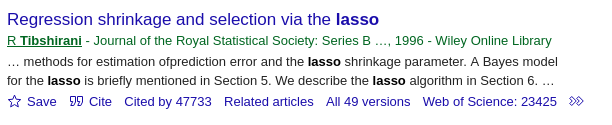
\includegraphics[width=0.8\linewidth]{lasso_citations}
        \caption{This paper on a method for sparse regression has 40,000 citations.}%
    \end{figure}
\end{frame}
\begin{frame}
    What will be new about this method?
    \begin{itemize}
        \item Fast and effective.
        \item Connections to other areas in modern linear algebra.
        \item Works for sparse linear regression and sparse PCA.
        \item Potential to be sped up in future work.
    \end{itemize}
\end{frame}

\begin{frame}
    \centering
    \huge
    {\color{gray}Bounds based on Polynomial Roots}
\end{frame}
\begin{frame}
    \frametitle{Motivation}
    \textbf{The following are the same.}
    \vspace{0.3in}
    \begin{columns}
        \begin{column}{0.48\textwidth}
            \begin{block}{Variational Characterization}
            \begin{equation*}
                \begin{aligned}
                    \max\quad & x^{\intercal}Ax\\
                    \st & x^{\intercal}x = 1\\
                \end{aligned}
            \end{equation*}
            \end{block}
        \end{column}
        \pause
        \begin{column}{0.48\textwidth}
            \begin{block}{Characteristic Polynomial}
            \[
                \max \{t : \det(tI - A) = 0\}.
            \]
            \end{block}
        \end{column}
    \end{columns}
\end{frame}
\begin{frame}
    \frametitle{Motivation}
    Whenever $A_1$ is PSD,
    \vspace{0.3in}
    \begin{columns}
        \begin{column}{0.48\textwidth}
            \begin{block}{QCQP}
            \begin{equation*}
                \begin{aligned}
                    \max\quad & x^{\intercal}A_0x\\
                    \st & x^{\intercal}A_1x = 1\\
                \end{aligned}
            \end{equation*}
            \end{block}
        \end{column}
        \begin{column}{0.48\textwidth}
            \begin{block}{Root}
            \[
                \max \{t : \det(tA_1 - A_0) = 0\}.
            \]
            \end{block}
        \end{column}
    \end{columns}
\end{frame}
\begin{frame}
    \frametitle{Idea}
    For $S \subseteq [n]$, the following are the same:
    \begin{columns}
        \begin{column}{0.48\textwidth}
            \begin{block}{QCQP}
            \begin{equation*}
                \begin{aligned}
                    \max\quad & x^{\intercal}A_0x\\
                    \st & x^{\intercal}A_1x = 1\\
                    \st & \supp(x) \subseteq S.
                \end{aligned}
            \end{equation*}
            \end{block}
        \end{column}
        \begin{column}{0.48\textwidth}
            \begin{block}{Root}
            \[
                \max \{t : \det(tA_1|_S - A_0|_S) = 0\}.
            \]
            \end{block}
        \end{column}
    \end{columns}
    We want to find the maximum of these programs over all $S$ with $|S| = k$.
\end{frame}
\begin{frame}
    \frametitle{Sparse Determinants}
    \begin{figure}[h]
        \centering
        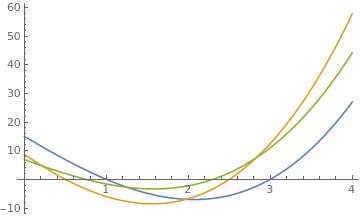
\includegraphics[width=0.6\linewidth]{univariates.png}
        \caption{Each subset of the columns has an associated polynomial.}%
        \label{fig:variety}
    \end{figure}
\end{frame}
\begin{frame}
    \frametitle{Sparse Determinants}
    \begin{figure}[h]
        \centering
        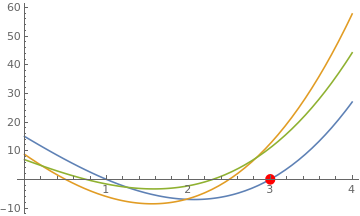
\includegraphics[width=0.6\linewidth]{univariates_root.png}
        \caption{We want the largest out of all of these roots.}%
        \label{fig:variety}
    \end{figure}
\end{frame}
\begin{frame}
    \frametitle{Sparse Determinants}
    \begin{figure}[h]
        \centering
        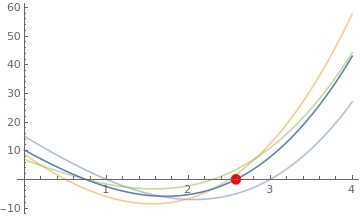
\includegraphics[width=0.6\linewidth]{univariates_average_root.png}
        \caption{Instead, take the average of all of these polynomials and find the maximum root of that.}%
        \label{fig:variety}
    \end{figure}
\end{frame}
\begin{frame}
    \frametitle{Sparse Determinants}
    A \emph{linear combination of minors} polynomial of degree $k$ is a polynomial in a symmetric matrix of indeterminants so that
    \[
        p(X) = \sum_{S \subseteq [n] : |S| = k}a_S\det(X|_S),
    \]
    Here $X|_S$ is the principal submatrix of $X$ indexed by the elements of $S$.
\end{frame}
\begin{frame}
    \frametitle{An Inequality}
    \begin{block}{Theorem}
        Let $p$ be an LPM polynomial with nonnegative coefficients.  If $A_1$ is PSD, then
        \begin{equation*}
            \begin{aligned}
                \max\quad & x^{\intercal}A_0x\\
                \st & x^{\intercal}A_1x = 1\\
                    &|\supp(x)| \le k.
            \end{aligned}
        \end{equation*}
        is at least 
        \[
            \eta = \max \{y : p(A_1y-A_0) = 0 \}.
        \]
    \end{block}
\end{frame}
\begin{frame}
    \frametitle{An Inequality}
    \begin{block}{Proof}
        Suppose that $p(A_1 \eta-A_0) = 0$, then there must be some $S$ so that 
        \[
            \det(\eta A_1|_S - A_0|_S) \le 0.
        \]
        This means that the maximum root of this polynomial must be at least $\eta$, so that the corresponding optimization problem has a solution that is at least $\eta$.
    \end{block}
\end{frame}
\begin{frame}
    \centering
    \huge
    {\color{gray}Applications of this Inequality}
\end{frame}
\begin{frame}
    \frametitle{Reminder of the Inequality}
    \begin{block}{Theorem}
        Let $p$ be an LPM polynomial with nonnegative coefficients.  If $A_1$ is PSD, then
        \begin{equation*}
            \begin{aligned}
                \max\quad & x^{\intercal}A_0x\\
                \st & x^{\intercal}A_1x = 1\\
                    &|\supp(x)| \le k.
            \end{aligned}
        \end{equation*}
        is at least 
        \[
            \eta = \max \{y : p(A_1y-A_0) = 0 \}.
        \]
    \end{block}
\end{frame}
\begin{frame}
    \frametitle{What do we do with this inequality?}
    \begin{itemize}
        \item Are there LPM polynomials that we can find the roots of quickly?
        \pause 
        \item Can we efficiently find a solution to the sparse QCQP that does at least as well as this result guarantees?
        \pause
        \item Is this inequality any good?
    \end{itemize}
\end{frame}
\begin{frame}
    \frametitle{What now?}
    \begin{itemize}
        \item \textbf{Are there LPM polynomials that we can find the roots of quickly?}
        \item Can we efficiently find a solution to the sparse QCQP that does at least as well as this result guarantees?
        \item Is this inequality any good?
    \end{itemize}
\end{frame}
\begin{frame}
    \frametitle{Characteristic Coefficients}
    Define
    \[
        c_n^k(Y) = \sum_{\top{S \subseteq [n]}{|S| = k}}  \det(Y|_S).
    \]
    \pause 
    This is an LPM polynomial with very simple coefficients.
\end{frame}
\begin{frame}
    \frametitle{Characteristic Coefficients}
    \begin{block}{Facts About Characteristic Coefficients}
        $c_n^k(Y)$ is sometimes called a \emph{characteristic coefficient}, since it is a coefficient of the characteristic polynomial of $Y$, i.e.
        \[
            \det(Y + tI) = \sum_{j=0}^n c_n^{n-j}(Y) t^j.
        \]
        \pause
        In particular, it is
        \begin{itemize}
            \item Basis invariant, so that $c_n^k(U^{\intercal} Y U) = c_n^k(Y)$ for any orthogonal matrix $U$.
            \pause
            \item Efficiently computable.
            \pause
            \item If $X$ is PSD, then $c_n^k(tX+Y)$ has only real roots for any $Y$.
        \end{itemize}
    \end{block}
\end{frame}
\begin{frame}
    \frametitle{Newton's Method for Real Rooted Polynomials}
    \begin{block}{Theorem}
        If $p(t)$ is a real rooted polynomial of degree $d$, then for large enough $t_0$, Newton's method converges to the maximum root of $p(t)$ in $O(d \log(t_0 / \epsilon))$ steps.
    \end{block}
    Interpolation lets me evaluate $p(t)$ at $d$ points, then apply Newton's method.
\end{frame}
\begin{frame}
    \frametitle{What now?}
    \begin{itemize}
        \item Are there LPM polynomials that we can find the roots of quickly?
            \begin{itemize}
                \item \textbf{Yes!}
            \end{itemize}
        \item Can we efficiently find a solution to the sparse QCQP that does at least as well as this result guarantees?
        \item Is this inequality any good?
    \end{itemize}
\end{frame}
\begin{frame}
    \frametitle{What now?}
    Two questions:
    \begin{itemize}
        \item Are there LPM polynomials that we can find the roots of quickly?
            \begin{itemize}
                \item Yes!
            \end{itemize}
        \item \textbf{Can we efficiently find a solution to the sparse QCQP that does at least as well as this result guarantees?}
            \only<2-> {
            \begin{itemize}
                \item Yes!
            \end{itemize}
            }
        \item \textbf{Is this inequality any good?}
            \only<2-> {
            \begin{itemize}
                \item Not really, but this can be fixed.
            \end{itemize}
            }
    \end{itemize}
    \pause
    Both of these will be resolved by introducing different coefficients.
\end{frame}
\begin{frame}
    \centering
    \huge
    {\color{gray}Conditioning}
\end{frame}
\begin{frame}
    \frametitle{Conditioning}
    \textbf{Idea:} Reduce the size of the support of $p$.

    For a LPM polynomial $p$, and $i \in [n]$, define the conditioning.
    \[
        p|_i(X) = \sum_{S : i \in S} a_S \det(X|_S).
    \]
    This has support strictly smaller than $p$.
\end{frame}
\begin{frame}
    \frametitle{Conditioning}
    \begin{theorem}
    For any LPM polynomial $p$ with nonnegative coefficients, there exists some $i$ so that
    \[
        \eta_{p|_i} \ge \eta_{p}.
    \]
    \end{theorem}
\end{frame}
\begin{frame}
    \frametitle{Conditioning}
    \begin{block}{Proof}
    Consider
        \begin{align*} 
        \sum_{i \in [n]} p|_{i}&=\sum_{i \in [n]} \sum_{i \in  S} a_S \det(X|_S)\\
                &=k\sum_{S} a_S \det(X|_S)\\
                &=kp
        \end{align*}
    \end{block}
\end{frame}
\begin{frame}
    \frametitle{Conditioning}
    \begin{block}{Proof}
    \[
        \sum_{i\in [n]}p|_i(\eta_p) = kp(\eta_p) = 0.
    \]
    \pause
    Therefore, for some $i$, $ p|_{i}(\eta_{p}) \le 0$.
    \pause
    This implies that the largest root of $p|_{i}$ is at least $\eta_{p}$.
    \end{block}
\end{frame}
\begin{frame}
    \frametitle{Computing Conditionings}
    \textbf{We want to compute}
    \[
        p|_i = \sum_{S : i \in S} a_S \det(X|_S).
    \]
    How can we do this?
\end{frame}
\begin{frame}
    \frametitle{Computing Conditionings}
    \textbf{Idea: } Notice that
    \begin{align*}
        \frac{\partial}{\partial X_{ii}} p(X) &= \sum_{S} a_S \frac{\partial}{\partial X_{ii}}  \det(X|_{S})\\
                               &= \sum_{S : i \in S} a_S \det(X|_{S \setminus i})
    \end{align*}
\end{frame}
\begin{frame}
    \frametitle{Computing Conditionings}
    Also, recall the Schur complement identity for determinants:
    \begin{align*}
        \det(X|_S) = X_{ii} \det((X \setminus i)|_{S \setminus i}),
    \end{align*}
    where 
    \[
        X \setminus i = X - \frac{1}{X_{ii}} X_i X_i^{\intercal}.
    \]
    Here, $X_i$ is the $i^{th}$ column of $X$.
\end{frame}
\begin{frame}
    \frametitle{Computing Conditionings}
    \begin{block}{Theorem}
        \[
            p|_i(X) = X_{ii} \frac{\partial}{\partial X_{ii}} p(X \setminus i).
        \]
    \end{block}
    When $p = c_n^k$, $\frac{\partial}{\partial X_{ii}} p(X) = c_{n-1}^{k-1}(X)$, so 
    \[
        p|_i(X) = X_{ii} c_{n-1}^{k-1}(X \setminus i).
    \]
\end{frame}
\begin{frame}
    \frametitle{Computing Conditionings}
    It's also true that if $p$ is LPM and $p(A_1 t - A_0)$ has real roots for all PSD $A_1$, then the same is true for $p|_i$.
\end{frame}
\begin{frame}
    \centering
    \huge
    {\color{gray}Algorithms}
\end{frame}
\begin{frame}
    \frametitle{An Algorithm for Sparse QCQPs}
    Putting it all together,
    \begin{algorithm}[H]
    \caption{The Greedy Conditioning Heuristic}
    \label{alg:greedy}
    \begin{algorithmic}
        \State $T \gets \varnothing$
        \For{$t = 1 \dots k$}
            \State $j \gets \argmax \eta_{p|_{T + j}}$
            \State $T \gets T + j$
        \EndFor

        \Return $T$
    \end{algorithmic}
    \end{algorithm}

    We have seen that this will always produce an answer which is at least $\eta_p$, and we have means of computing all of these things efficiently.
\end{frame}
\begin{frame}
    \begin{figure}[h]
        \centering
        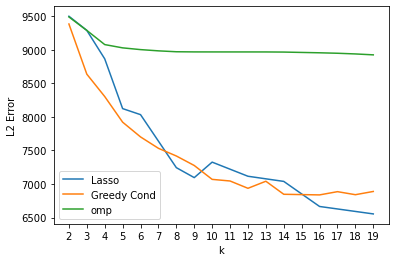
\includegraphics[width=0.8\linewidth]{superconductivity.png}
        \caption{Superconductivity. 81 Columns, 0.03 seconds at the maximum.}%
        \label{fig:superconductivity}
    \end{figure}
\end{frame}
\begin{frame}
    \begin{figure}[h]
        \centering
        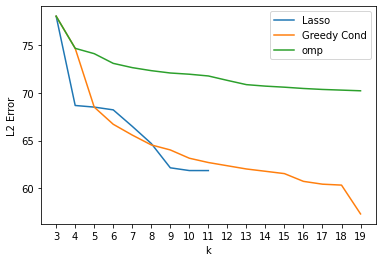
\includegraphics[width=0.8\linewidth]{violentcrime.png}
        \caption{Communities. 101 columns. Under 0.03 seconds at the maximum.}%
        \label{fig:name}
    \end{figure}
\end{frame}
\begin{frame}
    \tiny{
\begin{table}[H]
\begin{center}
    \begin{tabular}{c|c c c c c c}
        Dataset & Columns & $k$ & Found Value & Optimal Value & Gap & Time (s)\\
        \hline
        Wine & 13 & 5 & 3.43 & 3.43 & $<10^{-5}$ & $3\times 10^{-4}$\\
             &    & 10 & 4.45 & 4.59 & $0.03$ & $8\times 10^{-4}$\\
        \hline
        Pitprops & 13 & 5 & 3.40 & 3.40 & $<10^{-5}$ & $3\times 10^{-4}$\\
             &    & 10 & 3.95 & 4.17 & $0.05$ & $8\times 10^{-4}$\\
        \hline
        MiniBooNE & 50 & 5 & 4.99 & 5.00 & $<10^{-5}$ & 0.003\\
             &    & 10 & 9.99 & 9.99 & $<10^{-5}$ & 0.012\\
        \hline
        Communities & 101 & 5 & 4.51 & 4.86 & 0.07 & 0.02 \\
             &    & 10 & 8.71 & 8.82 & $0.013$ & 0.09\\
        \hline
        Arrythmia & 274 & 5 & 4.18 & 4.23 & 0.012 & 0.39\\
         & & 10 & 7.49 & 7.53 & 0.005 & 1.44
    \end{tabular}

\end{center}
\caption{A table describing the results of running our algorithm for sparse PCA on various datasets and values of $k$.  The gap is defined to be $\frac{\text{Optimal Value} - \text{Found Value}}{\text{Optimal Value}}$.}
\end{table}}
\end{frame}
\begin{frame}
    \frametitle{An Algorithm for Sparse QCQPs}
    Good news and bad news
    \begin{description}
        \item[Good] This already gives the accuracy competitive with LASSO and others that we saw at the beginning of the talk.
        \pause
        \item[Bad] Slow! Computing everything naively is 1000x slower than LASSO!
    \end{description}

    \pause
    We can speed it up by a lot by doing incremental computations: instead of recomputing characteristic coefficients, we will use efficient update formulas and diagonalization maintance.
\end{frame}
\begin{frame}
    \frametitle{Computing Characteristic Polynomials.}
    Let $X = QDQ^{\intercal}$ be the diagonalization of a matrix $X$, i.e.
    \begin{itemize}
        \item $Q$ is the orthogonal matrix whose columns are eigenvectors of $X$.
        \item $D$ is diagonal and its entries are eigenvalues of $X$.
    \end{itemize}
\end{frame}
\begin{frame}
    \frametitle{Computing Characteristic Polynomials.}
    $c_n^k(X)$ is given by the elementary symmetric polynomial in the eigenvalues of $X$:
    \[
        c_n^k(X) = \sum_{S \subseteq [n],|S| = k} \prod_{i \in S}\lambda_i,
    \]
    where the $\lambda_i$ are eigenvalues of $X$.
\end{frame}
\begin{frame}
    \frametitle{Computing Characteristic Polynomials.}
    If the diagonalization of $X$ is given, the characteristic coefficient can be computed in $O(nk)$ time using dynamic programming to compute the elementary symmetric polynomial in the eigenvalues.

    \textbf{Given a diagonalization of $X$, I can compute the characteristic coefficients of $X$ quickly.}
\end{frame}
\begin{frame}
    \frametitle{Computing Characteristic Polynomials.}
    \begin{block}{Theorem}
        Given a diagonalization of a matrix $X$, we can compute $p|_i(X)$  \emph{all} in $O(n^2 + kn\log(n))$ time.
    \end{block}
\end{frame}
\begin{frame}
    \frametitle{Computing Characteristic Polynomials.}
    We want to compute
    \[
        p|_i(X) = X_{ii} c_{n-1}^{k-1}(X - \frac{1}{X_{ii}}X_iX_i^{\intercal})?
    \]
    \textbf{Idea: } Use rank 1 updates instead of recomputing.
\end{frame}
\begin{frame}
    \frametitle{Computing Characteristic Polynomials.}
    Because $\frac{1}{X_{ii}}X_iX_i^{\intercal}$ is rank 1, the first order Taylor expansion gives an exact answer:
    \[
        c_{n-1}^{k-1}(X - \frac{1}{X_{ii}}X_iX_i^{\intercal}) = c_{n-1}^{k-1}(X)  - \frac{1}{X_{ii}}X_i^{\intercal}\nabla c_{n-1}^{k-1}(X)X_i.
    \]
    If we already have $c_{n-1}^{k-1}(X)$ for each $i$, we really just want to compute
    \[
        X_i^{\intercal}\nabla c_{n-1}^{k-1}(X)X_i.
    \]
\end{frame}
\begin{frame}
    \frametitle{Computing Characteristic Polynomials.}
    Because $\frac{1}{X_{ii}}X_iX_i^{\intercal}$ is rank 1, the first order Taylor expansion gives an exact answer:
    \[
        c_{n-1}^{k-1}(X - \frac{1}{X_{ii}}X_iX_i^{\intercal}) = c_{n-1}^{k-1}(X)  - \frac{1}{X_{ii}}X_i^{\intercal}\nabla c_{n-1}^{k-1}(X)X_i.
    \]
    If we already have $c_{n-1}^{k-1}(X)$ for each $i$, we really just want to compute
    \[
        X_i^{\intercal}{\color{red}\nabla c_{n-1}^{k-1}(X)}X_i.
    \]
\end{frame}
\begin{frame}
    \frametitle{Computing Characteristic Polynomials.}
    \textbf{Idea:} We can change basis because characteristic coefficients are basis invariant, so if $X = QDQ^{\intercal}$, then
    \[
        \nabla c_{n-1}^{k-1}(X) = Q\nabla c_{n-1}^{k-1}(D)Q^{\intercal},
    \]
    \textbf{$\nabla c_{n-1}^{k-1}(D)$ is a diagonal matrix.}
\end{frame}
\begin{frame}
    \frametitle{Computing Characteristic Polynomials.}
    \textbf{Idea:} We can change basis because characteristic coefficients are basis invariant, so
    \[
        X_i^{\intercal}\nabla c_{n-1}^{k-1}(X)X_i = X_i^{\intercal}Q\nabla c_{n-1}^{k-1}(D)Q^{\intercal}X_i,
    \]
    \pause
    Now, we use the fact that $Q$ is a matrix of eigenvectors, and $X_i$ is a column of $X$ to get
    \[
        X_i^{\intercal}Q = DQ_i^{\intercal},
    \]
    where $Q_i$ is a row of $Q$.
\end{frame}
\begin{frame}
    \frametitle{Computing Characteristic Polynomials.}
    The matrix-vector product
    \[
        Q^{*2}D^2\diag(\nabla c_{n-1}^{k-1}(D))
    \]
    computes the updates for \emph{all values of $i$ at the same time}, and it only takes $O(n^2)$ time to do, given $\nabla c_{n-1}^{k-1}(D)$.
\end{frame}
\begin{frame}
    \frametitle{Computing Characteristic Polynomials.}
    \[
        \diag(\nabla c_{n-1}^{k-1}(D))
    \]
    Can be computed, for any diagonal matrix $D$ in $O(kn\log(n))$ time using dynamic programming.
\end{frame}
\begin{frame}
    \frametitle{Returning to our algorithm}
    \begin{algorithm}[H]
    \caption{The Greedy Conditioning Heuristic}
    \label{alg:greedy}
    \begin{algorithmic}
        \State $T \gets \varnothing$
        \For{$t = 1 \dots k$}
            \State $j \gets \argmax \eta_{p|_{T + j}}$ \COMMENT{\textbf{(*)}}
            \State $T \gets T + j$
        \EndFor

        \Return $T$
    \end{algorithmic}
    \end{algorithm}
    In round 1, can compute (*) in roughly time $O(n^2)$ if $k$ is much smaller than $n$.
\end{frame}
\begin{frame}
    \frametitle{Returning to our algorithm}
    \begin{block}{Theorem}
        For any given matrix $X$, we can compute diagonalizations of $X$ in $O(n^3)$ time.
        Given a diagonalization of $X$, we can compute a diagonalization of $X - \rho vv^{\intercal}$ in $O(n^{\omega})$ time, where $\omega$ is the fast matrix multiplication constant.
    \end{block}
    After each round, we can replace $X$ by $X \setminus j$, which allows us to finish every round in roughly $O(n^{\omega})$ time.
\end{frame}
\begin{frame}
    \frametitle{Returning to our algorithm}
    \begin{block}{Theorem}
        The algorithm can be completed in roughly $O(n^3)$ time.
    \end{block}
    In theory, this can be brought down to $O(n^{\omega})$ time using fast matrix multiplication and recent results on diagonalization.
\end{frame}
\begin{frame}
    \centering
    \huge
    {\color{gray}Concrete Aspects For Sparse Regression}
\end{frame}
\begin{frame}
    \frametitle{Example}
    Sparse regression is a sparse QCQP where
    \[
        A_0 = \hat{b}\hat{b}^{\intercal},
    \]
    \[
        A_1 = A^{\intercal}A,
    \]
    where $\hat{b} = A^{\intercal}b$.
\end{frame}
\begin{frame}
    \frametitle{Example}
    Plugging this into our expression for sparse linear regression, we want to compute
    \[
        \eta = \max \{y : p(A^{\intercal}Ay-\hat{b}\hat{b}^{\intercal}) = 0 \},
    \]
    for an LPM polynomial $p$.

    \pause
    When $y = 0$, 
    \[
        p(A^{\intercal}Ay-\hat{b}\hat{b}^{\intercal}) = p(\hat{b}\hat{b}^{\intercal}) = 0,
    \]
    because $\hat{b}\hat{b}^{\intercal}$ is rank 1.


\end{frame}
\begin{frame}
    \frametitle{Example}
    In fact, when $y=0$, this vanishes with multiplicity $d-1$! The polynomial actually must have the form
    \[
        p(A^{\intercal}Ay-\hat{b}\hat{b}^{\intercal}) = y^{d-1}(k_1y+k_2),
    \]
    for some constants $k_1$ and $k_2$.
\end{frame}
\begin{frame}
    \frametitle{Example}
    \begin{block}{An explicit formula for linear regression}
        \[
            \eta = \frac{p(A^{\intercal}A+\hat{b}\hat{b}^{\intercal})}{p(A^{\intercal}A)} - 1.
        \]
    \end{block}
\end{frame}
\begin{frame}
    \frametitle{Example}
    Sanity check: when $k = n$, this becomes
    \[
        \eta = \frac{\det(A^{\intercal}A+\hat{b}\hat{b}^{\intercal})}{\det(A^{\intercal}A)} - 1.
    \]
    \pause
    This turns out to be exactly the formula for the optimal error in ordinary least squares regression, and can be seen as a version of Cramer's rule for solving a system of linear equations.
\end{frame}
\begin{frame}
    \frametitle{Example}
    \begin{block}{An explicit formula for linear regression}
        \[
            \eta = \frac{p(A^{\intercal}A+\hat{b}\hat{b}^{\intercal})}{p(A^{\intercal}A)} - 1.
        \]
    \end{block}
    \pause
    This same expression appears in other places!
\end{frame}
\begin{frame}
    \frametitle{A Probabilistic Interpretation}
    \[
        p(X) = \sum_{S \subseteq [n] : |S| = k} a_S\det(X|_S).
    \]
    
    \pause
    For a subset $S \subseteq [n]$ with $|S| = k$,
    \[
        \pi(S) = \frac{a_S\det(A^{\intercal}A|_S)}{p(A^{\intercal}A)}.
    \]
    This is a probability distribution over subsets of size $k$.
\end{frame}
\begin{frame}
    \frametitle{A Probabilistic Interpretation}
    \[
        \pi(S) = \frac{a_S\det(A^{\intercal}A|_S)}{p(A^{\intercal}A)}
    \]
    
     is called \emph{weighted determinantal point process}. This selects a random subset of $[n]$ proportional to the determinant of $\det(A^{\intercal}A|_S)$.

     \pause 
     DPPs are very popular in machine learning because they model \emph{diversity}; a subset is more likely to be chosen if its columns are very far apart.
\end{frame}

\begin{frame}
    \frametitle{A Probabilistic Interpretation}
    \begin{block}{A Probabilistic Interpretation}
    \[
        \eta = \frac{\det(A^{\intercal}A+\hat{b}\hat{b}^{\intercal})}{\det(A^{\intercal}A)} - 1 = \E[\ell(A_S, b)].
    \]
    \end{block}
    where $\ell(A, b) = \max \{\|b\|^2 - \|Ax - b\|_2^2 : x \in \R^k\}$ the norm of the projection of $b$ onto the column space of $A$, and $S$ is chosen from a weighted DPP.
\end{frame}
\begin{frame}
    \frametitle{Conditioning and Determinantal Point Processes}
    \textbf{Why is it called conditioning?}
    Recall that if we are working with sparse regression, for any LPM polynomial $p$,
    \[
        \eta_p = \E[\ell(A_S, b)],
    \]
    where the expectation is taken with respect to a weighted DPP.

    Then,
    \[
        \eta_{p|_i} = \E[\ell(A_S, b)|i \in S],
    \]
\end{frame}
\begin{frame}
    \[
        p|_i(X) = \sum_{S : i \in S} a_S \det(X|_S).
    \]
    \pause
    Questions
    \begin{itemize}
        \item Is $p|_i$ better than $p$ for some $i$?
        \item Can we compute $\eta|_{p|_i}$ quickly?
    \end{itemize}
\end{frame}
\begin{frame}
    \centering
    \huge
    {\color{gray}Conical Programming and Hyperbolicity Cones}
\end{frame}
\begin{frame}
\frametitle{Concrete Question}
What happens if $A_1$ is not PSD? What happens if I have multiple constraints?
\end{frame}
\begin{frame}
\frametitle{Stability}
\begin{block}{Recall}
    If $X$ is PSD, then $c_n^k(tX+Y)$ has only real roots for any $Y$.
\end{block}
This is what allows us to use Newton's method to find maximal roots.
\end{frame}
\begin{frame}
\frametitle{Stability}
\begin{block}{Definition}
    A polynomial $p$ in a symmetric matrix of variables is said to be PSD-stable if for any PSD $X$, and symmetric matrix $Y$, $p(tX+Y)$ has only real roots.
\end{block}
\pause
Characteristic coefficients are PSD stable.
\pause 
Conditionings of PSD stable polynomials are PSD stable.
\end{frame}

\begin{frame}
\frametitle{Stability}
PSD stability has a lot of nice properties.
\begin{block}{Theorem}
    If, for any symmetric matrix $Y$, $p(tI+Y)$ has real roots, and $p$ does not vanish at any PSD matrix, then $p$ is PSD stable.
\end{block}
\pause
\begin{block}{Theorem}
    If $p$ is an LPM polynomial, then $p$ is PSD stable if and only if for any diagonal matrix $D$, $p(tI+D)$ is real rooted.
\end{block}
\end{frame}

\begin{frame}
\frametitle{Stability}
We now come to the definition of the hyperbolicity cone:
\begin{block}{Definition}
    If $p$ is PSD stable, then the open hyperbolicity cone of $p$ is the largest connected set containing $I$ on which  $p$ does not vanish. The (closed) hyperbolicity cone of $p$, $H(p)$, is the closure of the open hyperbolicity cone.
\end{block}
\begin{block}{Theorem}
    The hyperbolicity cone of $p$ is convex, and $\log(p)$ is a self-concordant barrier function for the hyperbolicity cone.
\end{block}
\end{frame}
\begin{frame}
    \begin{block}{Theorem}
        For any $A_1$ so that $A_1$ has some PSD $k\times k$ submatrix, and any PSD-stable LPM polynomial $p$,
        \begin{equation}
            \begin{aligned}
                \max\quad & \tr(A_0X)\\
                \st & \tr(A_1X) = 1\\
                    & X \in H(p)\\
            \end{aligned}
        \end{equation}
        is a lower bound on the corresponding sparse QCQP.
        If $A_1$ is PSD, this agrees with $\eta$.
    \end{block}
\end{frame}
\begin{frame}
    \begin{block}{Theorem}
        For any $A_1$ so that $A_1$ has some PSD $k\times k$ submatrix, and any PSD-stable LPM polynomial $p$,
        \[
            \eta = \max \{t : A_1t + A_0 \in H(p) \}
        \]

        is a lower bound on the corresponding sparse QCQP.
        If $A_1$ is PSD, this agrees with the earlier definition of $\eta$.
    \end{block}
\end{frame}
\begin{frame}
    We can also deal with two constraints, as long as one is PSD.

    Consider 2-constraint sparse QCQP 
    \begin{equation}
        \begin{aligned}
            \max\quad & x^{\intercal}A_0x\\
            \st & x^{\intercal}A_1x = 1\\
                & x^{\intercal}A_2x = 1\\
                & \|x\|_0 \le k
        \end{aligned}
    \end{equation}
    Then, 
    \[
        \max \{s+t : sA_1+tA_2+A_0 \in H(p)\}
    \]
    is a lower bound on the optimum value of this sparse QCQP.
\end{frame}

\begin{frame}
    \frametitle{Conclusions}
    \begin{itemize}
        \item Fast algorithm based on the roots of polynomials.
        \item Effective on practical problems.
        \item Connections to probability and algebra.
    \end{itemize}
\end{frame}
\begin{frame}
    \frametitle{Open Questions}
    \begin{itemize}
        \item Can we prove that this is effective on some interesting instances?
        \item Are there smarter ways of reducing the size of the supports for our polynomials?
        \item Are there faster sampling based methods for sparse regression?
        \item Are there other LPM polynomials with interesting coefficients we can compute efficiently?
    \end{itemize}
    
\end{frame}
\end{document}
